\section{Results}
\label{sec:results}
All numbers are relative RMSE against random sampling with the same $n$ (below 1 is better), geometric mean over benchmarks, with 95\% hierarchical-bootstrap intervals (Section~\ref{sec:protocol}); 13 benchmarks for random and stronger-target splits and the 7 Open LLM Leaderboard benchmarks for held-out organisations. For scale, random sampling with $n=100$ has an RMSE of about 3--5 accuracy points on most benchmarks (Appendix Table~\ref{tab:abs}); much of this is a component shared by all targets of a split, because they use one coreset.

\begin{table}[t]
\caption{Relative RMSE vs.\ random sampling (geometric mean over benchmarks; 95\% CI). Rows above the rule are baselines; ``ours'' are the components proposed here; AUTO is source-only pseudo-shift tuning. Best entries per column in the interpolation settings are the learned predictors; in the extrapolation setting they are the recalibrated/residual-corrected estimators. The held-out-organisation column covers 7 benchmarks, the others 13. Full results for all five budgets are in Appendix Table~\ref{tab:full}.}
\label{tab:main}
\centering\scriptsize\setlength{\tabcolsep}{3.2pt}
\begin{tabular}{lcccccc}
\toprule
 & \multicolumn{2}{c}{Random split} & \multicolumn{2}{c}{Held-out organisations} & \multicolumn{2}{c}{Stronger targets (extrapolation)} \\
 & $n$=25 & $n$=100 & $n$=25 & $n$=100 & $n$=25 & $n$=100 \\
\midrule
Random sampling & 1.00\,\scriptsize(1.00--1.00) & 1.00\,\scriptsize(1.00--1.00) & 1.00\,\scriptsize(1.00--1.00) & 1.00\,\scriptsize(1.00--1.00) & 1.00\,\scriptsize(1.00--1.00) & 1.00\,\scriptsize(1.00--1.00) \\
Difficulty-stratified sampling & 0.83\,\scriptsize(0.79--0.88) & 0.83\,\scriptsize(0.79--0.87) & 0.83\,\scriptsize(0.76--0.89) & 0.86\,\scriptsize(0.80--0.91) & 0.82\,\scriptsize(0.78--0.87) & 0.82\,\scriptsize(0.78--0.87) \\
Random + linear calibration & 0.67\,\scriptsize(0.57--0.76) & 0.79\,\scriptsize(0.74--0.83) & 0.61\,\scriptsize(0.49--0.75) & 0.77\,\scriptsize(0.69--0.85) & 0.95\,\scriptsize(0.85--1.07) & 1.07\,\scriptsize(0.95--1.19) \\
Random + ridge regression & 0.61\,\scriptsize(0.50--0.72) & 0.73\,\scriptsize(0.63--0.83) & 0.53\,\scriptsize(0.41--0.67) & 0.67\,\scriptsize(0.56--0.81) & 1.12\,\scriptsize(0.94--1.32) & 1.65\,\scriptsize(1.37--1.96) \\
Anchor points (weighted mean) & 0.78\,\scriptsize(0.68--0.89) & 1.08\,\scriptsize(0.91--1.28) & 0.82\,\scriptsize(0.67--1.03) & 1.21\,\scriptsize(0.95--1.63) & 0.90\,\scriptsize(0.65--1.30) & 1.34\,\scriptsize(0.90--2.07) \\
Anchor points + IRT (tinyBenchmarks-style) & 0.58\,\scriptsize(0.47--0.71) & 0.83\,\scriptsize(0.66--1.07) & 0.48\,\scriptsize(0.40--0.58) & 0.67\,\scriptsize(0.58--0.81) & 1.02\,\scriptsize(0.85--1.22) & 1.40\,\scriptsize(1.11--1.73) \\
D-optimal items + IRT (info-based) & 0.70\,\scriptsize(0.55--0.92) & 1.01\,\scriptsize(0.79--1.33) & 0.53\,\scriptsize(0.41--0.67) & 0.77\,\scriptsize(0.63--0.96) & 1.01\,\scriptsize(0.85--1.20) & 1.62\,\scriptsize(1.33--1.98) \\
Random + IRT (pure) & 0.65\,\scriptsize(0.55--0.75) & 0.78\,\scriptsize(0.70--0.86) & 0.57\,\scriptsize(0.46--0.69) & 0.71\,\scriptsize(0.64--0.80) & 1.08\,\scriptsize(0.90--1.29) & 1.54\,\scriptsize(1.35--1.79) \\
Random + IRT-AIPW & 0.78\,\scriptsize(0.73--0.82) & 0.80\,\scriptsize(0.77--0.83) & 0.77\,\scriptsize(0.71--0.83) & 0.80\,\scriptsize(0.74--0.86) & 0.78\,\scriptsize(0.73--0.84) & 0.82\,\scriptsize(0.77--0.87) \\
VA-PPS + IRT-AIPW & 0.78\,\scriptsize(0.72--0.87) & 0.82\,\scriptsize(0.77--0.89) & 0.75\,\scriptsize(0.68--0.83) & 0.77\,\scriptsize(0.71--0.82) & 0.76\,\scriptsize(0.69--0.84) & 0.88\,\scriptsize(0.78--0.98) \\
VA-PPS + IRT (pure) & 0.65\,\scriptsize(0.54--0.79) & 0.82\,\scriptsize(0.69--1.00) & 0.54\,\scriptsize(0.45--0.64) & 0.69\,\scriptsize(0.64--0.76) & 1.02\,\scriptsize(0.86--1.20) & 1.51\,\scriptsize(1.30--1.76) \\
VA-PPS + Cal-IRT (ours) & 0.69\,\scriptsize(0.63--0.75) & 0.75\,\scriptsize(0.71--0.80) & 0.65\,\scriptsize(0.59--0.72) & 0.74\,\scriptsize(0.69--0.80) & 0.70\,\scriptsize(0.64--0.76) & 0.76\,\scriptsize(0.70--0.82) \\
VA-PPS + ShrinkCal-IRT (ours) & 0.64\,\scriptsize(0.58--0.72) & 0.71\,\scriptsize(0.66--0.77) & 0.58\,\scriptsize(0.51--0.65) & 0.68\,\scriptsize(0.62--0.74) & 0.80\,\scriptsize(0.71--0.90) & 0.88\,\scriptsize(0.82--0.93) \\
AUTO (pseudo-shift, minimax) & 0.68\,\scriptsize(0.59--0.76) & 0.75\,\scriptsize(0.71--0.80) & 0.62\,\scriptsize(0.51--0.73) & 0.73\,\scriptsize(0.67--0.78) & 0.77\,\scriptsize(0.68--0.87) & 0.82\,\scriptsize(0.74--0.91) \\
AUTO (pseudo-shift, mean) & 0.66\,\scriptsize(0.55--0.76) & 0.72\,\scriptsize(0.67--0.77) & 0.58\,\scriptsize(0.45--0.72) & 0.70\,\scriptsize(0.63--0.77) & 0.81\,\scriptsize(0.71--0.95) & 0.87\,\scriptsize(0.76--0.99) \\
\bottomrule
\end{tabular}

\end{table}

\paragraph{Interpolation: learned predictors help a lot.}
When targets are drawn at random from the same population as the sources, predictors beat random sampling by wide margins at small budgets: with $n=25$, ridge regression on the coreset responses reaches 0.61 (0.50--0.72), anchors with IRT imputation 0.58 (0.47--0.71), and pure IRT 0.65 (0.55--0.75). Gains shrink as $n$ grows (0.73--0.83 at $n=100$), as expected when the baseline error falls like $n^{-1/2}$. With held-out organisations the picture is the same or slightly stronger (anchors+IRT 0.48 at $n=25$). Rankings improve too: Spearman's $\rho$ rises by $+0.05$ to $+0.13$ at $n=25$ (Appendix Table~\ref{tab:spearman}). Difficulty-stratified sampling, which needs no model at all, lowers RMSE by about 17\% (0.83, CI 0.79--0.88) at every budget and in every split type, and wins on all benchmarks (Appendix Table~\ref{tab:wins}).

\paragraph{Extrapolation: predictors become worse than random sampling.}
When the targets are the strongest quarter of the models, every method that predicts from the source population without a correction degrades. At $n=100$, pure IRT has relative RMSE 1.54 (1.35--1.79), ridge 1.65 (1.37--1.96), anchors+IRT 1.40 (1.11--1.73) and D-optimal items+IRT 1.62 (1.33--1.98); they beat random sampling on only 1--3 of 13 benchmarks (Appendix Table~\ref{tab:wins}). The error is systematic: Table~\ref{tab:bias} shows a mean signed error of $-5$ accuracy points, accounting for about three quarters of the MSE. Rank correlation also falls below that of random sampling ($-0.08$ to $-0.16$ in $\rho$; Appendix Table~\ref{tab:spearman}). The anchor-weighted mean, which is design-based but uses cluster sizes from the source population, is also no better than random sampling at $n=100$ (1.34, CI 0.90--2.07) in this setting.

\begin{figure}[t]
\centering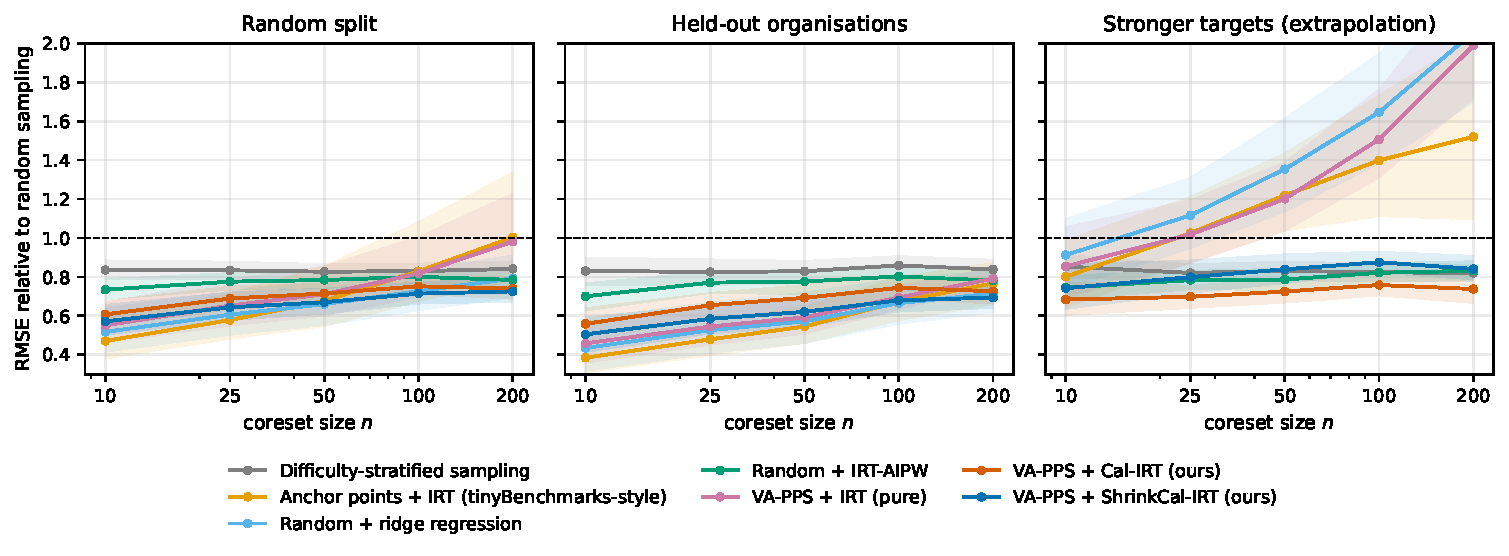
\includegraphics[width=\linewidth]{figs/curves.pdf}
\caption{Relative RMSE vs.\ random sampling as a function of coreset size, per split type (shaded: 95\% CI). The vertical axis is clipped at 2.0; pure-prediction methods continue upwards in the right panel.}
\label{fig:curves}
\end{figure}

\paragraph{Residual correction or recalibration restores robustness.}
Model-assisted (AIPW) estimators remain design-unbiased under any shift: IRT-AIPW with uniform sampling has 0.78 (0.73--0.84) at $n=25$ and 0.82 (0.77--0.87) at $n=100$ under extrapolation and beats random sampling on all 13 benchmarks at both budgets. Cal-IRT with VA-PPS improves on this: 0.70 (0.64--0.76) and 0.76 (0.70--0.82), 13/13 wins, and is better than IRT-AIPW in paired comparisons by 11\% and 8\% (ratio 0.89 and 0.92 with intervals excluding 1; Appendix Table~\ref{tab:pairs}). Under interpolation, Cal-IRT keeps most of the gain (0.69 and 0.75 for random splits), but remains behind the best uncorrected predictors at small $n$ (paired ratio vs.\ ridge 1.14 at $n=25$, CI 1.00--1.34). Its bias under extrapolation is $-0.5$ points versus $-5.2$ for the uncalibrated IRT with the same design (Table~\ref{tab:bias}). ShrinkCal-IRT trades in the other direction: it recovers most of the interpolation advantage (0.64/0.71 for random splits, within the intervals of ridge) and costs 15\% relative to Cal-IRT under extrapolation (0.80/0.88, still better than random sampling on 13/13). No method dominates: the choice between Cal-IRT and ShrinkCal-IRT is a choice about how much extrapolation to expect.

\begin{table}[t]
\caption{Signed error and its share in the MSE at $n=100$: average over benchmarks of the mean signed error $\hat a_t-a_t$ over target models (accuracy points) and bias$^2$/MSE pooled over runs. A shared coreset produces some common-mode error even for unbiased methods.}
\label{tab:bias}
\centering\scriptsize\setlength{\tabcolsep}{3pt}
\begin{tabular}{lcccccc}
\toprule
 & \multicolumn{2}{c}{Random split} & \multicolumn{2}{c}{Held-out organisations} & \multicolumn{2}{c}{Stronger targets (extrapolation)} \\
 & mean err (pts) & bias$^2$/MSE & mean err (pts) & bias$^2$/MSE & mean err (pts) & bias$^2$/MSE \\
\midrule
Random sampling & -0.03 & 28\% & -0.08 & 24\% & -0.09 & 42\% \\
Difficulty-stratified sampling & -0.00 & 4\% & +0.05 & 3\% & -0.13 & 18\% \\
Random + linear calibration & +0.02 & 3\% & -0.02 & 3\% & -2.61 & 64\% \\
Random + ridge regression & +0.11 & 4\% & -0.05 & 3\% & -5.66 & 76\% \\
Anchor points (weighted mean) & -0.35 & 25\% & -1.79 & 26\% & -1.64 & 25\% \\
Anchor points + IRT (tinyBenchmarks-style) & +0.38 & 8\% & -0.20 & 5\% & -5.04 & 73\% \\
D-optimal items + IRT (info-based) & +0.65 & 11\% & -0.44 & 11\% & -5.83 & 77\% \\
Random + IRT (pure) & -0.03 & 4\% & -0.17 & 5\% & -5.23 & 75\% \\
Random + IRT-AIPW & -0.01 & 4\% & +0.02 & 2\% & -0.31 & 18\% \\
VA-PPS + IRT-AIPW & +0.03 & 3\% & -0.04 & 2\% & -0.07 & 14\% \\
VA-PPS + IRT (pure) & +0.17 & 6\% & -0.16 & 4\% & -5.15 & 75\% \\
VA-PPS + Cal-IRT (ours) & -0.04 & 3\% & -0.08 & 2\% & -0.48 & 18\% \\
VA-PPS + ShrinkCal-IRT (ours) & -0.02 & 3\% & -0.11 & 3\% & -1.50 & 31\% \\
AUTO (pseudo-shift, minimax) & +0.01 & 4\% & -0.10 & 3\% & -1.32 & 40\% \\
AUTO (pseudo-shift, mean) & -0.05 & 3\% & -0.08 & 3\% & -1.69 & 45\% \\
\bottomrule
\end{tabular}

\end{table}

\paragraph{Designs matter much less than estimators.}
Holding the estimator fixed, difficulty stratification changes RMSE by $\le4\%$ for IRT-based estimators, and VA-PPS adds at most 5--7\% over stratification, significantly so only in some columns (Appendix Table~\ref{tab:design}; e.g.\ Cal-IRT, VA-PPS vs.\ stratified: 0.96 at $n=25$ and 0.95 at $n=100$ with held-out organisations, 0.93 at $n=25$ under extrapolation, but 0.98--0.99 elsewhere with intervals covering 1). The pure Neyman allocation ($\lambda=1$) is a poor design for estimators that use the Horvitz--Thompson weights alone: the weighted mean with VA-PPS $\lambda=1$ is 9--47\% worse than stratified sampling, and VA-PPS $\lambda=1$ with IRT-AIPW is slightly worse than with $\lambda=0.5$ (0.88 vs 0.78 at $n=100$ under extrapolation; Appendix Table~\ref{tab:abl}). Information-based (D-optimal) item selection, which concentrates items in a few directions of latent space, is worse than random or stratified items for the same estimators in our setting. The IRT dimension ($d\in\{2,4,8\}$) matters little for the corrected estimators; larger $d$ is slightly worse under extrapolation.

\paragraph{Pseudo-shift tuning does not buy robustness.}
Tuning the (design, estimator) pair on pseudo-shifts of the source models (AUTO) does reasonably in the interpolation settings (e.g.\ 0.68/0.75 at $n=25/100$ for random splits, minimax) but is 8--11\% worse than fixed Cal-IRT under extrapolation (paired ratio 1.11, CI 1.04--1.18, at $n=25$; 1.08, CI 1.02--1.15, at $n=100$), and 17--31\% of its minimax choices there are uncorrected predictors (pure IRT, plug-in or ridge; Appendix Table~\ref{tab:auto}), which fail on the real shift. Holding out the top quarter of the \emph{sources} produces a milder gap than the real extrapolation, so the inner validation under-estimates the bias. We view this as a caution against validating shift-robustness only by within-source splits.

\paragraph{Shift severity.}
In a smaller additional run (10 seeds, $n\in\{25,100\}$, four designs; Appendix~\ref{app:shift}) we varied which models are targets: the strongest 10\% or 50\% of models, or the weakest 25\%. Uncorrected predictors fail in every direction of extrapolation, and most when the sources are only the weaker half: at $n=100$ pure IRT is 1.16 (1.04--1.36) of random-sampling RMSE for the strongest-10\% targets and 2.07 (1.77--2.49) for strongest-50\%, and for the weakest-25\% targets they over-predict by 8--9 points (relative RMSE 2.1). Cal-IRT is below 1 in all four settings at both budgets, but for the weakest-25\% targets its intervals include 1 (0.90, 0.77--1.06 at $n=25$; 0.92, 0.81--1.05 at $n=100$) and so does IRT-AIPW's, so we cannot claim a gain over random sampling there; difficulty-stratified sampling (0.92 and 0.90) is the only method whose interval stays at or below 1.


\paragraph{Number of source models.}
In a further run on 7 benchmarks (10 seeds, $n\in\{25,100\}$, stratified and VA-PPS designs) we kept only $m\in\{20,50,100\}$ randomly chosen source models (Appendix~\ref{app:src}). With $m=20$, all model-based methods are clearly weaker, and under extrapolation difficulty-stratified sampling (0.79 at $n=25$, 0.83 at $n=100$) is better than all of them (Cal-IRT 0.86 and 0.94, intervals covering 1 at $n=100$); with $m=50$ Cal-IRT is already at 0.76 / 0.85 and with all sources 0.68 / 0.73 under extrapolation. Interpolation gains of uncorrected predictors also need $m\gtrsim50$ (ridge 0.71 / 0.56 / 0.52 at $n=25$ for $m=20/50/100$). The same figures are in a table in the appendix; note that for the HELM benchmarks the number of available source models is below 100, so $m=100$ equals the full source set there.
